%BEGIN COPYPASTE EL INFORME DEL INFO
\documentclass[10pt, a4paper,english,spanish]{article}
\usepackage{subfig}

\parindent=20pt
\parskip=8pt
\usepackage[width=15.5cm, left=3cm, top=2.5cm, height= 24.5cm]{geometry}

\usepackage{ccfonts,eulervm} 
\usepackage[T1]{fontenc}
\usepackage{epigraph}
\usepackage{amsmath}
\usepackage{amsfonts}
\usepackage{amssymb}
\usepackage{fancyhdr}
\usepackage[activeacute, spanish]{babel}
\usepackage{cancel}
\usepackage[utf8]{inputenc}
\usepackage{algorithm}
\usepackage{algpseudocode}
\usepackage{afterpage}
\usepackage{caratula}
\usepackage{url}
\usepackage{fancyhdr}
\usepackage{listings}
\usepackage{ulem}
\usepackage{dashrule}
\usepackage{pdflscape}

\floatname{algorithm}{Algoritmo}

\newtheorem{theorem}{Teorema}[section]
\newtheorem{lemma}[theorem]{Lema}
\newtheorem{proposition}[theorem]{Proposici\'on}
\newtheorem{corollary}[theorem]{Corolario}

\newcommand{\Var}{\textbf{var }}
\newcommand{\True}{\textbf{true }}
\newcommand{\False}{\textbf{false }}
\newcommand{\Break}{\textbf{break }}
\newcommand{\Continue}{\textbf{continue }}
\newcommand{\Param}{\textbf{param }}

\newenvironment{proof}[1][Demostraci\'on]{\begin{trivlist}
\item[\hskip \labelsep {\bfseries #1}]}{\end{trivlist}}
\newenvironment{definition}[1][Definici\'on]{\begin{trivlist}
\item[\hskip \labelsep {\bfseries #1}]}{\end{trivlist}}
\newenvironment{example}[1][Ejemplo]{\begin{trivlist}
\item[\hskip \labelsep {\bfseries #1}]}{\end{trivlist}}
\newenvironment{remark}[1][Observaci\'on]{\begin{trivlist}
\item[\hskip \labelsep {\bfseries #1}]}{\end{trivlist}}

\newcommand{\qed}{\nobreak \ifvmode \relax \else
      \ifdim\lastskip<1.5em \hskip-\lastskip
      \hskip1.5em plus0em minus0.5em \fi \nobreak
      \vrule height0.75em width0.5em depth0.25em\fi}

\parindent 0em
\algrenewcommand{\algorithmiccomment}[1]{//\textit{#1} }

\lstset{language=sql,numbers=left,tabsize=2,
	morekeywords={BEGIN,DECLARE,FOR,CREATE,PROCEDURE,RAISEERROR,EACH,ROW,BEFORE,AFTER}}

\pagestyle{fancy}
\thispagestyle{fancy}
\addtolength{\headheight}{1pt}
\lhead{BD - TP1}
\rhead{Grupo 1}
\cfoot{\thepage}
\renewcommand{\footrulewidth}{0.4pt}
\newcommand{\hblacksquare}{\hfill \blacksquare}
%FIN COPYPASTE EL INFORME DEL INFO
\begin{document}

\materia{Bases de datos}
\submateria{Primer Cuatrim\'estre de 2013}
\titulo{Trabajo Pr\'actico 1}
\subtitulo{Informe}
\grupo{Grupo 1}
\integrante{Pablo Gauna}{334/09}{gaunapablo@gmail.com}
\integrante{Juli\'an Sackmann}{540/09}{jsackmann@gmail.com}
\integrante{Manuel Ferreria}{199/10}{m.ferreria@gmail.com}
\integrante{Juan Pablo Darago}{272/10}{jpdarago@gmail.com}

\maketitle
\pagebreak

\tableofcontents
\pagebreak

\section{Introducci\'on}

En este trabajo pr\'actico se detalla el modelado realizado para
el \textit{backend}, en particular el subsistema de almacenamiento 
de datos mediante una base de datos relacional, de un sistema online
de reserva de pasajes de una aerol\'inea (problema referido en el enunciado 
bajo el nombre de \textit{booking}). Este problema consiste en mantener 
un sistema de reservas de pasajes de manera que el sistema en su totalidad 
(es decir m\'as alla del m\'odulo de base de datos implementado) permita a los
usuarios consultar y administrar reservas para pasajes de avi\'on.

En primer lugar se detalla el DER (Diagrama Entidad Relaci\'on) realizado
para este trabajo, junto con las limitaciones adicionales al modelo expresadas
en lenguaje coloquial. Posteriormente se detalla el Modelo Relacional derivado
del Diagrama Entidad Relaci\'on. Finalmente, se detalla la implementaci\'on
(mediate SQL) de 3 funcionalidades pedidas en el enunciado del trabajo pr\'actico.
Las mismas se detallan acordemente antes de mostrarse su implementaci\'on.


\section{Diagrama Entidad Relaci\'on}

\subsection{Diagrama en si}

A continuaci\'on incluimos el Diagrama Entidad Relaci\'on (DER) correspondiente
al dise\~no realizado para este trabajo. El mismo se puede ver en la Figura~\ref{fig::der}

\subsection{Restricciones adicionales en lenguaje coloquial}

Las siguientes limitaciones adicionales del Diagrama Entidad Relaci\'on mostrado anteriormente,
y que no se pueden detallar utilizando la notaci\'on misma, se incluyen a continuaci\'on.

\begin{enumerate}
	\item Un usuario puede tener hasta 3 ciudades favoritas (restricci\'on tomada del enunciado).
	\item Los \'indices de escala de un vuelo con escalas son consecutivos. Adicionalmente, se cumple
	que los aeropuertos de llegada y de salida es encadenan (esta restricci\'on, si bien no es necesaria
	la tomamos por simplicidad). Por ``se encadenan'' se entiende que, dada la escala con \'indice $i$
	ocurre que
	
	\begin{itemize}
		\item $i = 0$ o el aeropuerto de llegada de la escala $i-1$ es el aeropuerto de salida de
		la escala $i$.
		\item $i = n-1$ con $n$ la cantidad de escalas del viaje con escalas considerado, o el aeropuerto
		de llegada de la escala $i$ es el aeropuerto de salida de la escala $i+1$.
	\end{itemize}
	
	\item El vuelo esta determinado no solo por el vuelo en si sino tambi\'en por la clase del asiento. No se
	hacen otras distinciones entre asientos dentro de una misma clase ni nada por el estilo.
	\item El precio de un vuelo esta determinado por la clase y el viaje, para cada uno de los viajes que corresponden
	a las escalas del vuelo.
	\item La cantidad de reservas que tienen un vuelo bajo una cierta clase dentro de su lista (considerando escalas)
	no puede superar la cantidad de asientos disponibles para esa clase por la aeronave del vuelo.
    \item El usuario unicamente podr\'a tener cargada una tarjeta a la vez en el sistema.
\end{enumerate}

\subsection{Explicaci\'on de las decisiones tomadas}

A continuaci\'on detallamos el por qu\'e de algunas de las decisiones tomadas para el diseño del Diagrama Entidad Relaci\'on.

\begin{enumerate}
	\item Se consider\'o, como se explico anteriormente, que un viaje con escalas consiste de un viaje con varias escalas. El
	precio del viaje esta determinado por las relaci\'on entre los vuelos y clases de los asientos para cada uno los varios 
	vuelos del viaje, considerando adem\'as las tasas de llegada de los aeropuertos de llegada y salida.
	\item Se consider\'o preferible mantener la informaci\'on de los datos del viajero separado en cada reserva: La motivaci\'on
	de esto es que se ve por que el enunciado dice que una reserva puede ser realizada en nombre de otra persona (sin que esa
	persona sea un usuario registrado). Sin embargo, se le cobrar\'a a la persona registrada que realiz\'o la reserva (usando
	para ello los datos de cobro que tiene el usuario registrado). Si bien esto puede introducir redundancia cuando un usuario
	saca una reserva para si mismo, la otra opci\'on ser\'ia mantener valores especiales. Preferimos mantener una duplicaci\'on
	(se puede para ello usar un \textit{trigger} en los inserts) para mantener la simplicidad de los datos (las otras opciones
	consideradas implicaban mantener posibles nulls lo cual implicaba mantener una l\'ogica impl\'icita independiente de los
	datos guardados).
	\item Se decidi\'o que las multiples reservas de un usuario se modelan como reservas separadas. Sin embargo, una reserva
	puede comprender varios vuelos.
	\item Algunos de los detalles del enunciado, a falta de una especificaci\'on m\'as fina de los datos, se decidi\'o mantenerlos
	como campos de texto con contenido indeterminado. Ejemplos incluyen: la composici\'on de la tripulaci\'on, los datos de llegada
	y salida de un aeropuerto, los datos de la persona a nombre de cual se hace una reserva, la tasa de un aeropuerto, el modelo
	de una aeronave, etc.
	\item El tel\'efono de Aeropuerto se guarda como una entidad d\'ebil (y no como argumento) porque consideramos que un aeropuerto puede tener varios tel\'efonos (a diferencia de un usuario, de quien consideramos s\'olo uno).
    \item La unicidad de la tarjeta se desprende de simplificar el sistema de facturaci\'on, que no es la parte crucial de
    modelar. Se podria arreglar vinculando como atributo de la relacion en la reserva la tarjeta usada, pero
    agregaria complejidad convirtiendo la tarjeta en entidades fuertes que tienen que existir aunque el usuario no la use mas,
    como log historico.
\end{enumerate}


\section{Modelo Relacional}

A continuaci\'on detallamos el Modelo Relacional derivado del
Diagrama Entidad Relaci\'on realizado anteriormente. Una aclaraci\'on
de notaci\'on: PK corresponde al t\'ermino \textit{Primary Key} o \textit{Clave primaria},
CK corresponde a \textit{Candidate Key} o \textit{Clave candidata}, y FK corresponde a
\textit{Foreign Key} o \textit{Clave for\'anea}.

\begin{itemize}
	\item \textbf{Usuario}(\underline{idUsuario},username,nombre,apellido,telefono,fechaNacimiento,
	preferencias,\\ direccion,profesion,email,clavehash,\dashuline{idClase},
	\dashuline{idPaisNacimiento},\dashuline{idClaseFrecuente})
		\begin{itemize}
			\item \textit{PK:} idUsuario
			\item \textit{CK:} idUsuario,username
			\item \textit{FK:} idClase,idPaisNacimiento,idClaseFrecuente
		\end{itemize}
	\item \textbf{CiudadFavorita}\underline{(\dashuline{idUsuario},\dashuline{idCiudad})}
		\begin{itemize}
			\item \textit{PK = CK: } (idUsuario,idCiudad)
			\item \textit{FK:} idUsuario,idCiudad
		\end{itemize}
	\item \textbf{Tarjeta}(\underline{idTarjeta},nroTarjeta,empresa,\dashuline{idUsuario},codigoSeguridad,direccion)
		\begin{itemize}
			\item \textit{PK:} idTarjeta
			\item \textit{CK:} idTarjeta,(empresa,nroTarjeta)
			\item \textit{FK:} idTarjeta
		\end{itemize}
	\item \textbf{Reservas}(\underline{idReserva},\dashuline{idUsuario},tipoPago,fechaCaducidad, datosViajante,
		\dashuline{idVueloConEscalas}\\,\dashuline{idClase})
		\begin{itemize}
			\item \textit{PK = CK:} idReserva
			\item \textit{FK:} idUsuario,idVueloConEscalas,idClase
		\end{itemize}
	\item \textbf{VueloConEscalas}(\underline{idViajeConEscalas},\dashuline{idViajePartida},\\ \dashuline{idViajeLlegada})
		\begin{itemize}
			\item \textit{PK = CK:} idVueloConEscalas
			\item \textit{FK: } idViajePartida,idViajeLlegada
		\end{itemize}
	\item \textbf{PrecioParaClase}(\underline{\dashuline{idVueloConEscalas},\dashuline{isClase}},precio)
		\begin{itemize}
			\item \textit{PK = CK: } (idVueloConEscalas,idClase)
			\item \textit{FK: } idVueloConEscalas,idReserva
		\end{itemize}
	\item \textbf{Vuelos}(\underline{idVuelo},\dashuline{idAeronave},fechaSalida,fechaLlegada,\\ 
		\dashuline{idAeropuertoSalida},\dashuline{idAeropuertoLlegada})
		\begin{itemize}
			\item \textit{PK = CK:} idVuelo
			\item \textit{FK: } idAeronave,idAeropuertoSalida,idAeropuertoLlegada
		\end{itemize}
	\item \textbf{HaceEscalaEn}(\underline{\dashuline{idVueloConEscalas},\dashuline{idVuelo}},NumeroEscala)
		\begin{itemize}
			\item \textit{PK:} (idVueloConEscalas,idVuelo)
			\item \textit{CK:} (idVueloConEscalas,idVuelo)
			\item \textit{FK:} idVuelo,idVueloConEscalas
		\end{itemize}
	\item \textbf{Aeropuertos}(\underline{idAeropuerto},tasa,opcionesTransporte, nombre, \dashuline{idCiudad})
		\begin{itemize}
			\item \textit{PK: } idAeropuerto
			\item \textit{CK: } nombre
			\item \textit{FK: } idCiudad
		\end{itemize}
	\item \textbf{TelefonoAeropuerto} \underline{(\dashuline{idAeropuerto},numero)}
		\begin{itemize}
			\item \textit{PK = CK: } (idAeropuerto,numero)
			\item \textit{FK: } idAeropuerto
		\end{itemize}
	\item \textbf{Aeronaves}(\underline{idAeronave},tripulacion,millas,modelo,\dashuline{idPaisOrigen})
		\begin{itemize}
			\item \textit{PK = CK: } idAeronave
			\item \textit{FK: } idPaisOrigen
		\end{itemize}
	\item \textbf{Paises}(\underline{idPais},nombre)
		\begin{itemize}
			\item \textit{PK: } idPais
			\item \textit{CK: } idPais, nombre
		\end{itemize}
	\item \textbf{Ciudades}(\underline{idCiudad},nombre,\dashuline{idPais})
		\begin{itemize}
			\item \textit{PK: } idCiudad
			\item \textit{CK: } idCiudad, nombre
			\item \textit{FK: } idPais
		\end{itemize}
	\item \textbf{Clases}(\underline{idClase},nombre)
		\begin{itemize}
			\item \textit{PK: } idClase
			\item \textit{CK: } idClase, nombre
		\end{itemize}
	\item \textbf{DisponeDeAsientos}(\underline{\dashuline{idAeronave},\dashuline{idClase}},asientos)
		\begin{itemize}
			\item \textit{PK = CK: } (idAeronave,idClase)
			\item \textit{FK: } idClase, idAeronave	
		\end{itemize}
	\item \textbf{CiudadesFavoritas}(\underline{\dashuline{idUsuario},\dashuline{idCiudad}})
		\begin{itemize}
			\item \textit{PK = CK: } (idUsuario,idCiudad)
			\item \textit{FK: } idUsuario, idCiudad	
		\end{itemize}
\end{itemize}


\section{Funcionalidad}

\begin{itemize}
	\item Primera funcionalidad:
		\begin{itemize}
			\item Enunciado: Mediante SQL escribir una consulta para obtener el nombre, apellido y nombre
			identificatorio de aquellos pasajeros que han viajado a todos los paises cubertis por la l\'inea
			a\'erea en los \'ultimos 5 a\~nos.

			\item Resoluci\'on:

			\lstinputlisting{primeraConsulta.sql}
		\end{itemize}
	\item Segunda funcionalidad:
		\begin{itemize}
			\item Enunciado: Controlar mediante alguna restricci\'on que un usuario no pueda realizar
			reservas que se superpongan en el tiempo. La \'unica excepci\'on que se permite consiste en
			que un usuario puede realizar a lo sumo dos reservas para la misma fecha de viaje entre los
			mismos aeropuertos de origen y destino, siempre que la fecha de partida no se encuentre dentro
			de los pr\'oximos 7 d\'ias.
			\item Resultado: Vamos a utilizar un \textit{trigger}:

			\lstinputlisting{segundaConsulta.sql}
		\end{itemize}
	\item Tercera funcionalidad:
		\begin{itemize}
			\item Enunciado: Implementaci\'on de alguna restricci\'on adicional que surga del dise\~no.			
			\item Resultado: Decidimos implementar la siguiente restricci\'on:

			\begin{quotation}
				Para cada viaje, la cantidad de asientos reservados para ese viaje (considerando tambi\'en los vuelos
				que no reservaron directamente sino que es solamente una escala en su viaje) para una clase determinada 
				no supera la cantidad de asientos para esa misma clase en la aeronave.
			\end{quotation}

			Esta restricci\'on la implementamos mediante un \textit{trigger} en la inserci\'on de una reserva. 
			
			\lstinputlisting{terceraConsulta.sql}
		\end{itemize}
\end{itemize}



\newpage
\begin{landscape}
	\begin{figure}[H]
		\caption{Diagrama Entidad Relaci\'on correspondiente al dise\~no del trabajo pr\'actico}
		\label{fig::der}
		\centering
		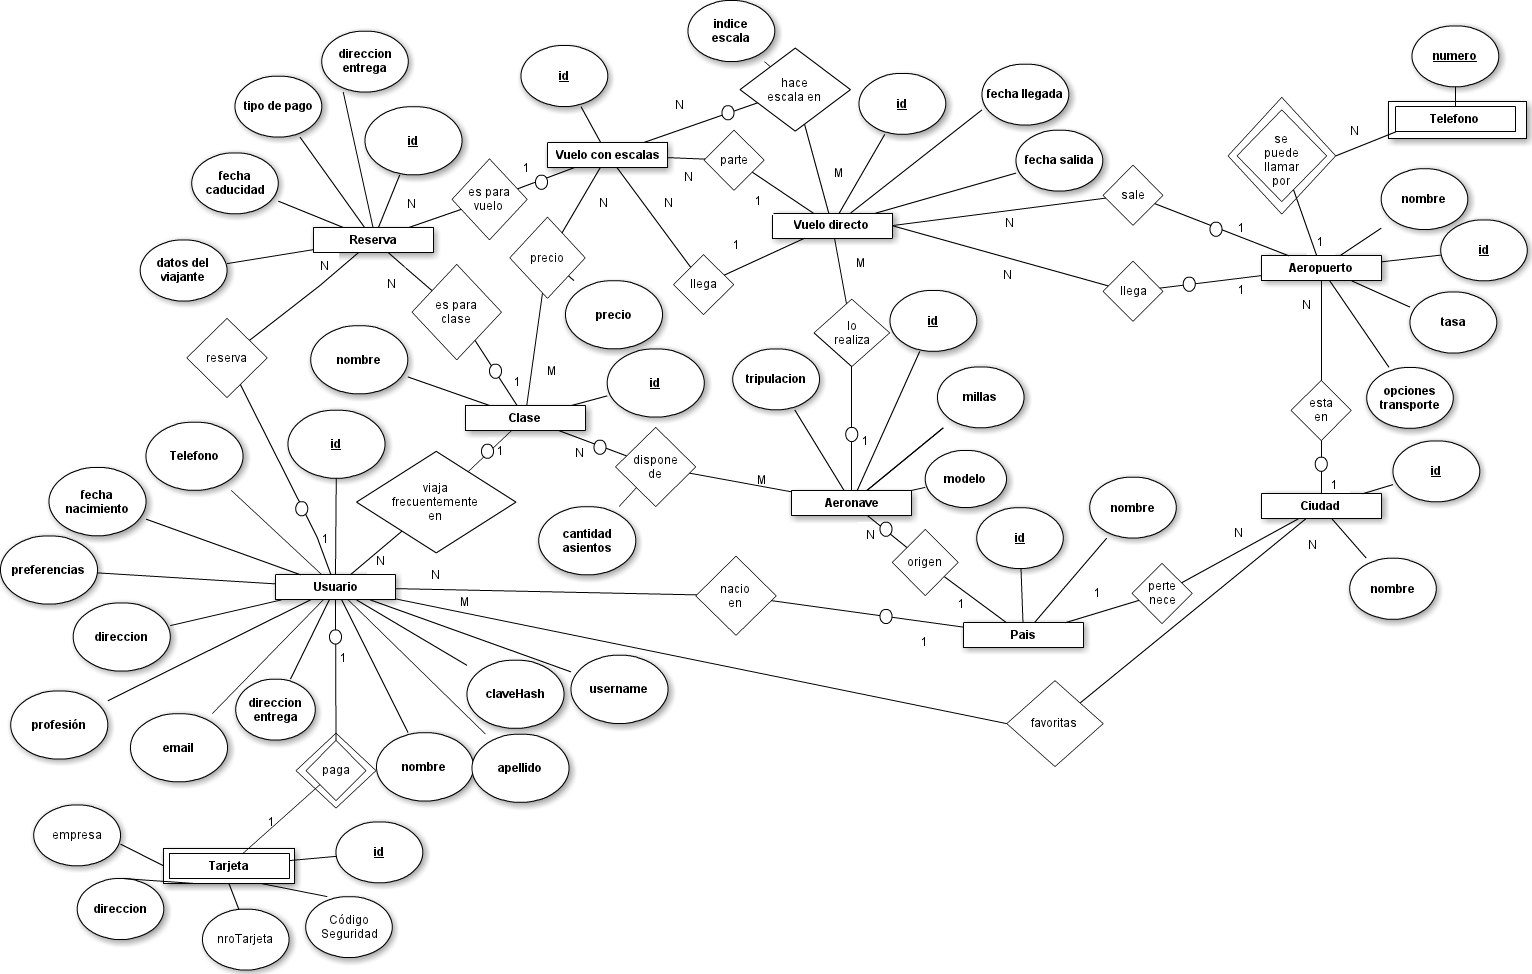
\includegraphics[width=1.3\textwidth]{der.png}
	\end{figure} 
\end{landscape}

\end{document}
